\documentclass{article}
\usepackage{amsmath}
\usepackage{amsfonts}
\usepackage{minted}
\usepackage{graphicx}
\graphicspath{ {./} }
\title{Intro to Computer Science Assignment 8}
\date{2017-11-08}
\author{Yiping Deng}
\begin{document}
\maketitle
\paragraph{1.}
\subparagraph{a.} Truth Table 1\\
\begin{center}
        \begin{tabular}{ |c|c|c|c|}
            \hline
            A & B & $C_{in}$ & $A \oplus B \oplus C_{in}$ \\
            \hline
            1 & 1 & 1 & 1 \\
            1 & 1 & 0 & 0 \\
            1 & 0 & 1 & 0 \\
            1 & 0 & 0 & 1 \\
            0 & 1 & 1 & 0 \\
            0 & 1 & 0 & 1 \\
            0 & 0 & 1 & 1 \\
            0 & 0 & 0 & 0 \\
            \hline
        \end{tabular}
\end{center}
Truth Table 2 \\
\begin{center}
    \begin{tabular} { |c|c|c|c|}
        \hline
        A & B & $C_{in}$ & $(A \land B) \lor (C \land (A \oplus B))$ \\
        \hline
        1 & 1 & 1 & 1 \\
        1 & 1 & 0 & 1 \\
        1 & 0 & 1 & 1 \\
        1 & 0 & 0 & 0 \\
        0 & 1 & 1 & 1 \\
        0 & 1 & 0 & 0 \\
        0 & 0 & 1 & 0 \\
        0 & 0 & 0 & 0 \\
        \hline
    \end{tabular}
\end{center}

\begin{align*}
    S &= A \oplus B \oplus C_{in} \\
    &= (A \land B \land C) \lor  (A \land \neg B \land \neg C) \lor \\
    &(\neg A \land B \land \neg C) \lor (\neg A \land \neg B \land C) \\
    C_{out} &= (A \land B) \lor (C_{in} \land (A \oplus B)) \\
    &=(A \lor B \lor C) \land (\neg A \lor \neg B \lor C) \lor \\
    &(\neg A \lor B \lor \neg C) \land (A \lor \neg B \lor \neg C) \\
\end{align*}
\subparagraph{b.}
Just read from the truths table
\begin{align*}
    S &= A \oplus B \oplus C_{in} \\
    &= (\neg A \lor \neg B \lor C_{out}) \land (\neg A \lor B \lor \neg C) \land \\
    &(A \lor \neg B \lor \neg C) \land (A \lor B \lor C) \\
    C_{out} &= (A \land B) \lor (C_{in} \land (A \oplus B)) \\
    &= (A \lor B) \land (A \lor C) \land (B \lor C)
\end{align*}
\subparagraph{c.}
also from the truth table
\begin{align*}
    S &= (A \uparrow B \uparrow C) \uparrow (A \uparrow \neg B \uparrow \neg C) \uparrow \\
    &(\neg A \uparrow B \uparrow \neg C) \uparrow (\neg A \uparrow \neg B \uparrow \neg C) \\
    C_{out} &= (A \uparrow B) \uparrow (A \uparrow C) \uparrow (B \uparrow C) \\
\end{align*}
\subparagraph{d.}
the diagram\\
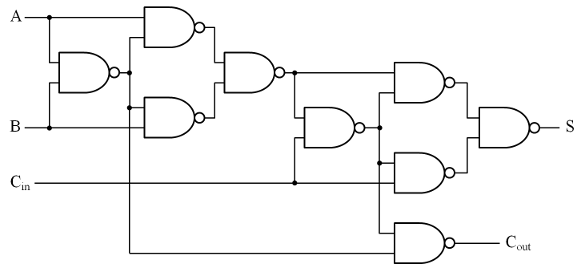
\includegraphics[scale=0.5]{full_adder.png}
\paragraph{2.} Code
\subparagraph{a)} implementing $bin$ function below
\subparagraph{b)} implementing in the following code, use Haskell to draw truth table
\subparagraph{c)} implementing accordingly
\subparagraph{d)} same, implementing accordingly
\inputminted{Haskell}{code.hs}
\end{document}

